\documentclass[final,t]{beamer}
\mode<presentation>
\usetheme{Purdue}

\setbeamerfont{itemize}{size=\normalsize}
\setbeamerfont{itemize/enumerate body}{size=\normalsize}
\setbeamerfont{itemize/enumerate subbody}{size=\normalsize}

\usepackage{times}
\usepackage{amsmath,amsthm, amssymb, latexsym}
\usepackage{exscale}
%\boldmath
\usepackage{booktabs, array}
%\usepackage{rotating}
\newenvironment{lisp}{\begin{tt}\begin{tabular}[t]{l}}{\end{tabular}\end{tt}}
\usepackage[english]{babel}
\usepackage[latin1]{inputenc}
\usepackage[orientation=landscape,size=custom,width=135.46667,height=101.6,scale=1.5]{beamerposter}
\listfiles
%\graphicspath{{figures/}}
% Display a grid to help align images
%\beamertemplategridbackground[1cm]

\title{\Huge Learning Physically-Instantiated Game Play Through Visual
Observation}
\author{Andrei Barbu, Siddharth Narayanaswamy, and Jeffrey Mark Siskind}
\institute[School of ECE]{School of Electrical and Computer Engineering}
\date[Apr. 25 , 2009]{Apr. 25 , 2009}

\usepackage{xspace}
\makeatletter
\DeclareRobustCommand\onedot{\futurelet\@let@token\@onedot}
\newcommand{\Prolog}{\mbox{\textsc{Prolog}}}
\newcommand{\Progol}{\mbox{\textsc{Progol}}}
\newcommand{\OpenCV}{\textsc{OpenCV}}
\def\@onedot{\ifx\@let@token.\else.\null\fi\xspace}
\def\eg{{e.g}\onedot} \def\Eg{{E.g}\onedot}
\def\ie{{i.e}\onedot} \def\Ie{{I.e}\onedot}
\def\cf{{c.f}\onedot} \def\Cf{{C.f}\onedot}
\def\etc{{etc}\onedot}
\def\vs{{vs}\onedot}
\def\wrt{w.r.t\onedot}
\def\dof{d.o.f\onedot}
\def\etal{{et al}\onedot}
\makeatother

\begin{document}
\begin{frame}{}
  \begin{columns}[t]
    \begin{column}{.3\linewidth}
      \begin{block}{Introduction}
	\begin{itemize}
	\item goal is to emulate a 2-year-old child
	\item an integrated robotics system for learning to play board games
	\item learn a full set of \alert{rules}; learn to play, not to
	  play well
	\item learn the initial board, legal-move generator, and
	  outcome predicate
	\item two robots play a board game, while a third watches and takes
	  over
	\item fully automatic with no human intervention
	\item no communication between the robots
	\end{itemize}
      \end{block}

      \begin{block}{Why games, and why learning?}
	\begin{itemize}
	\item games are an idealized version of the real world
	\item most AI cannot deal with real-world complexity
	\item children learn from observation
	\item not only when rules are unavailable, \cf\ Social Learning
	  Theory
	\item have you read the rules for board games you've played?
	\end{itemize}
      \end{block}

      \begin{block}{Experimental setup}
	\textbf{Robots}
	\begin{itemize}
	\item custom robots with a 4-DOF arm, two fingers, and two eyes
	\item eyes on a 1-DOF pendulum arm that rotates around the game
	\item each eye can pan/tilt independently
	\item mounted in a custom housing
	\item parts primarily from Lynxmotion, enhanced with custom parts
	  to provide greater support for the arm and eyes and increased
	  efficacy of operation
	\end{itemize}

	\vskip1ex
	\textbf{Computer Vision}
	\begin{itemize}
	\item reconstruct the game state from visual information
	\item must detect the board itself; this is a calibration
	  step done once on startup where 9 ellipses arranged in a
	  grid are found
	\item \OpenCV\ ellipse finder is used with multiple
	  thresholds and voting in order to detect Xs, Os, and empty
	  board positions
	\end{itemize}

	\vskip1ex
	\textbf{Games}
	\begin{itemize}
	\item off-the-shelf game hardware, but judiciously chosen to
	  simplify robotic manipulation
	\item depressions in the board provide for easy piece placement
	\item large, easy-to-grab pieces
	\item \alert{Tic-Tac-Toe} with standard rules learned
	\item \alert{Hexapawn}; three pawns on opposing sides; win by
	  queening, capture, or force an inability to move
	\item learned 5 variants of Hexapawn: regular, forward diagonal moves,
	  forward and backward diagonal moves, vertical backward moves,
	  vertical backward and sideways moves
	\end{itemize}
      \end{block}
    \end{column}

    \begin{column}{.3\linewidth}
      \begin{block}{Task}
	\centering{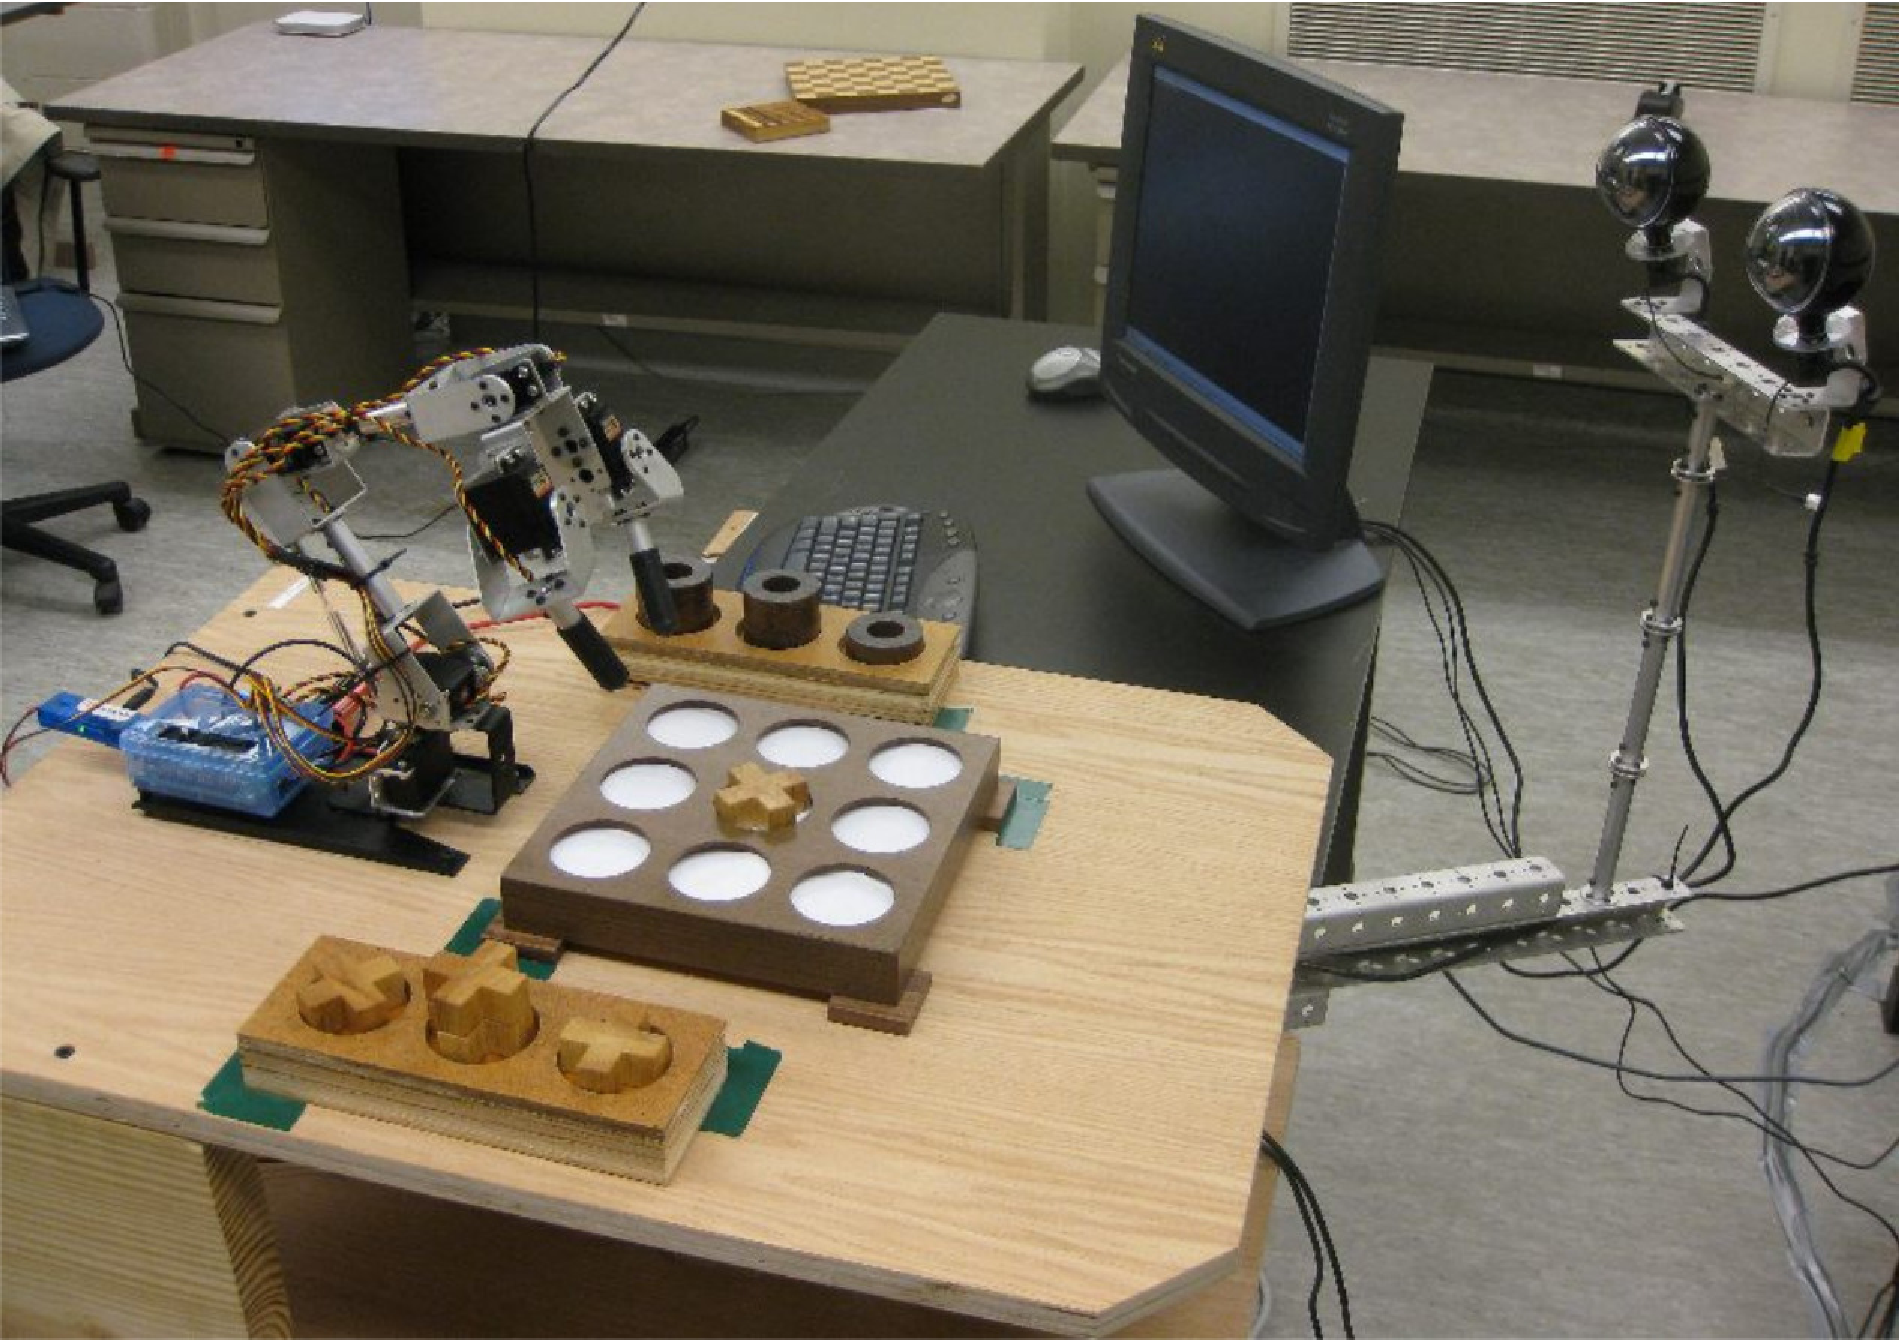
\includegraphics[width=0.960\linewidth]{orrorin}}
	\begin{figure}
	  \begin{scriptsize}
	    \begin{center}
	      \begin{displaymath}
    	   	\begin{array}{@{}lcr@{}}
    	   	  \left.\begin{tabular}{@{}c@{}c@{}c@{}c@{}c@{}}
    	   	    \begin{tabular}[t]{c}
    	   	      \resizebox{0.1\linewidth}{!}
		      {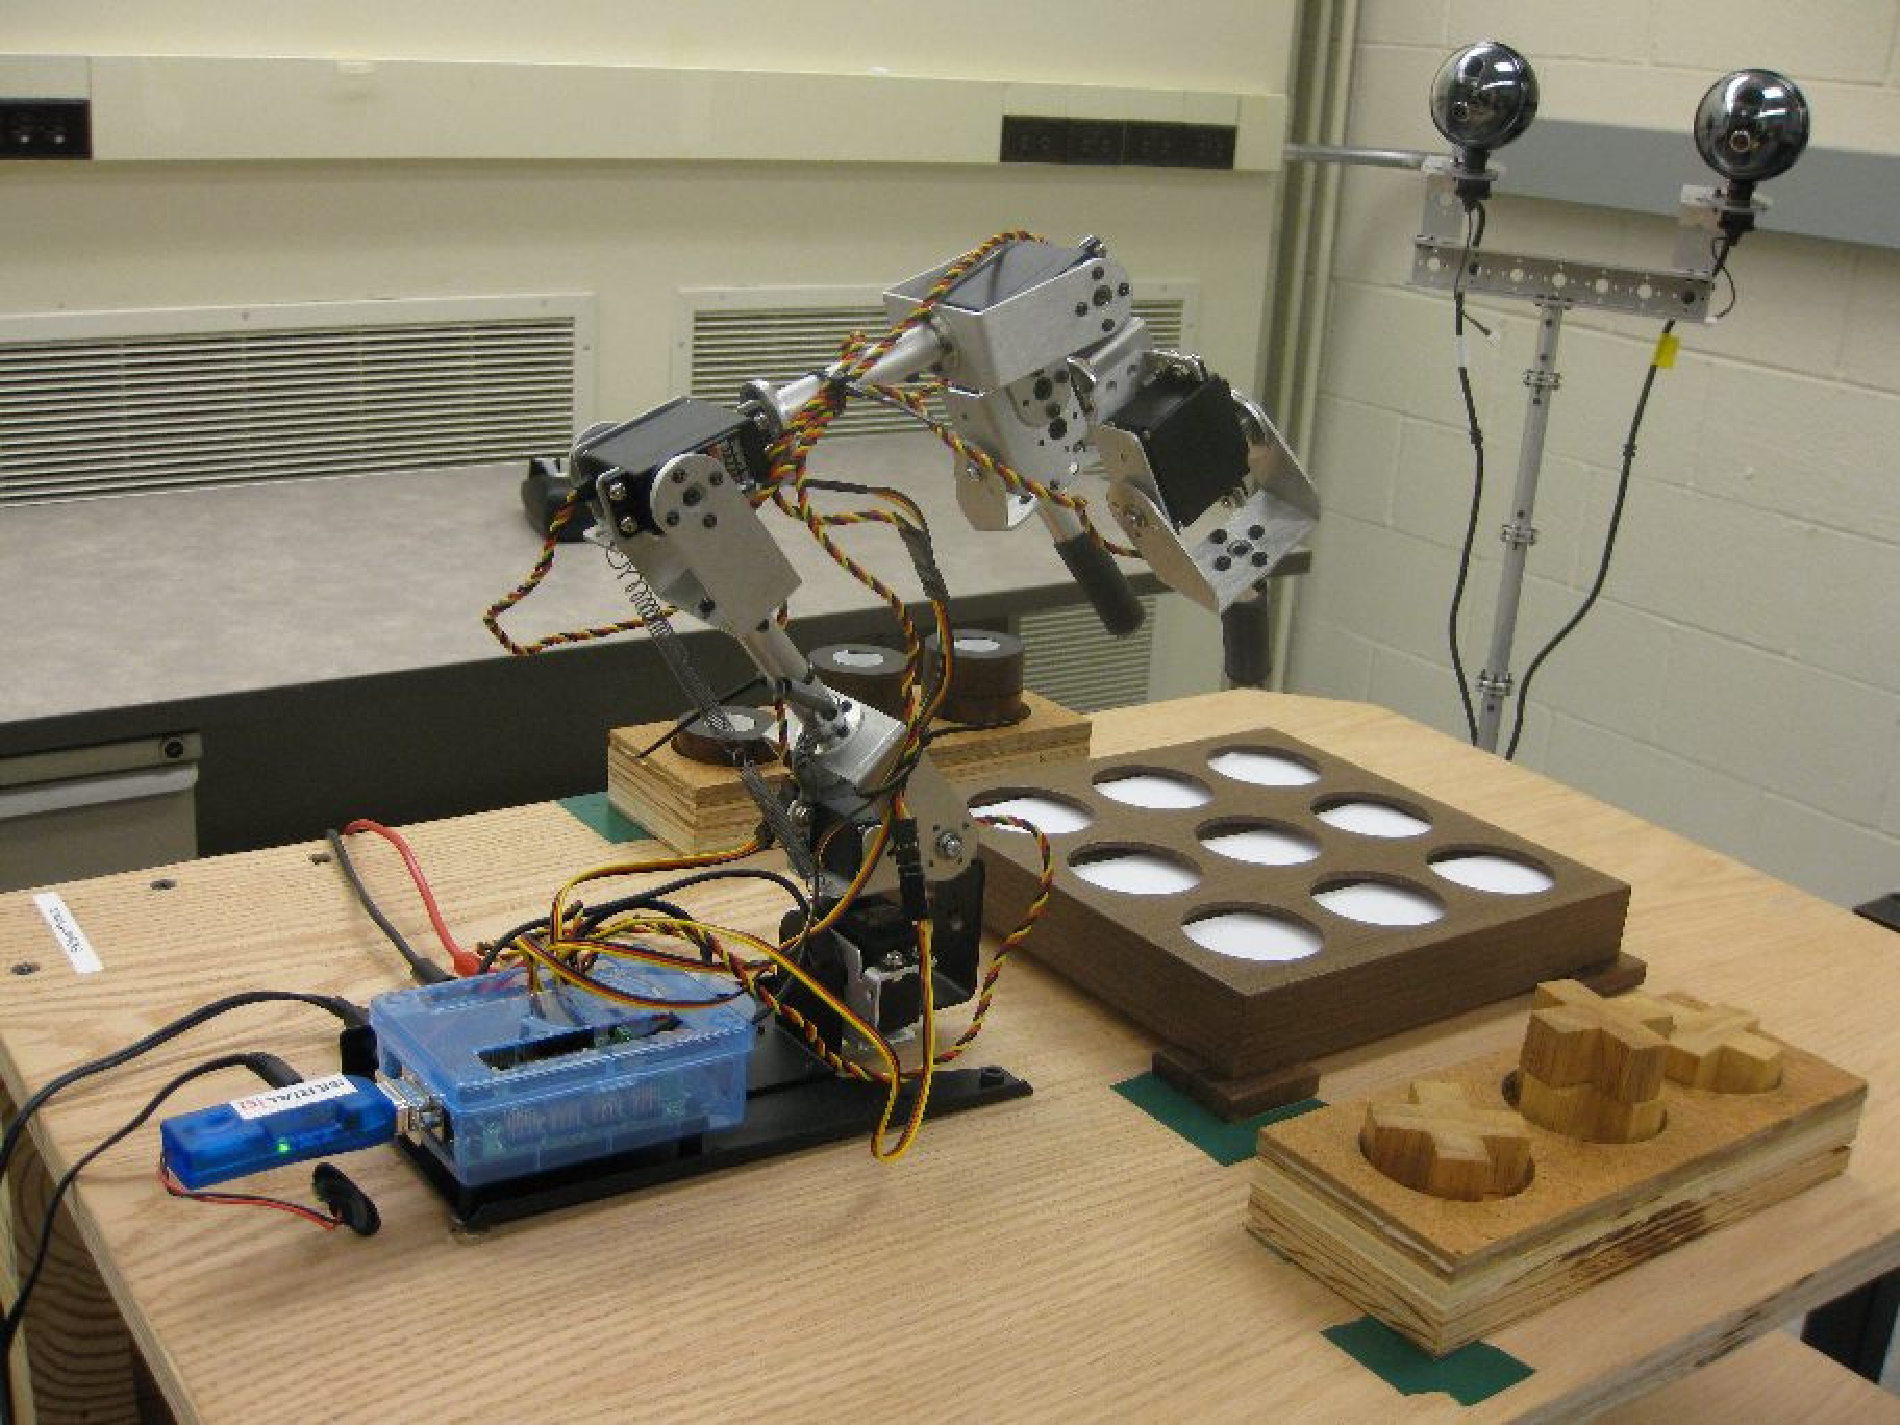
\includegraphics{sahelanthropus}}\\
    	   	      \textbf{protagonist}
    	   	    \end{tabular}&
    	   	    \raisebox{5ex}[0pt][0pt]{\begin{tabular}{@{}c@{}}
    	   		plays\\
    	   		\scalebox{2}{$\longrightarrow$}\\
    	   	    \end{tabular}}&
    	   	    \begin{tabular}[t]{c}
    	   	      \resizebox{0.1\linewidth}{!}{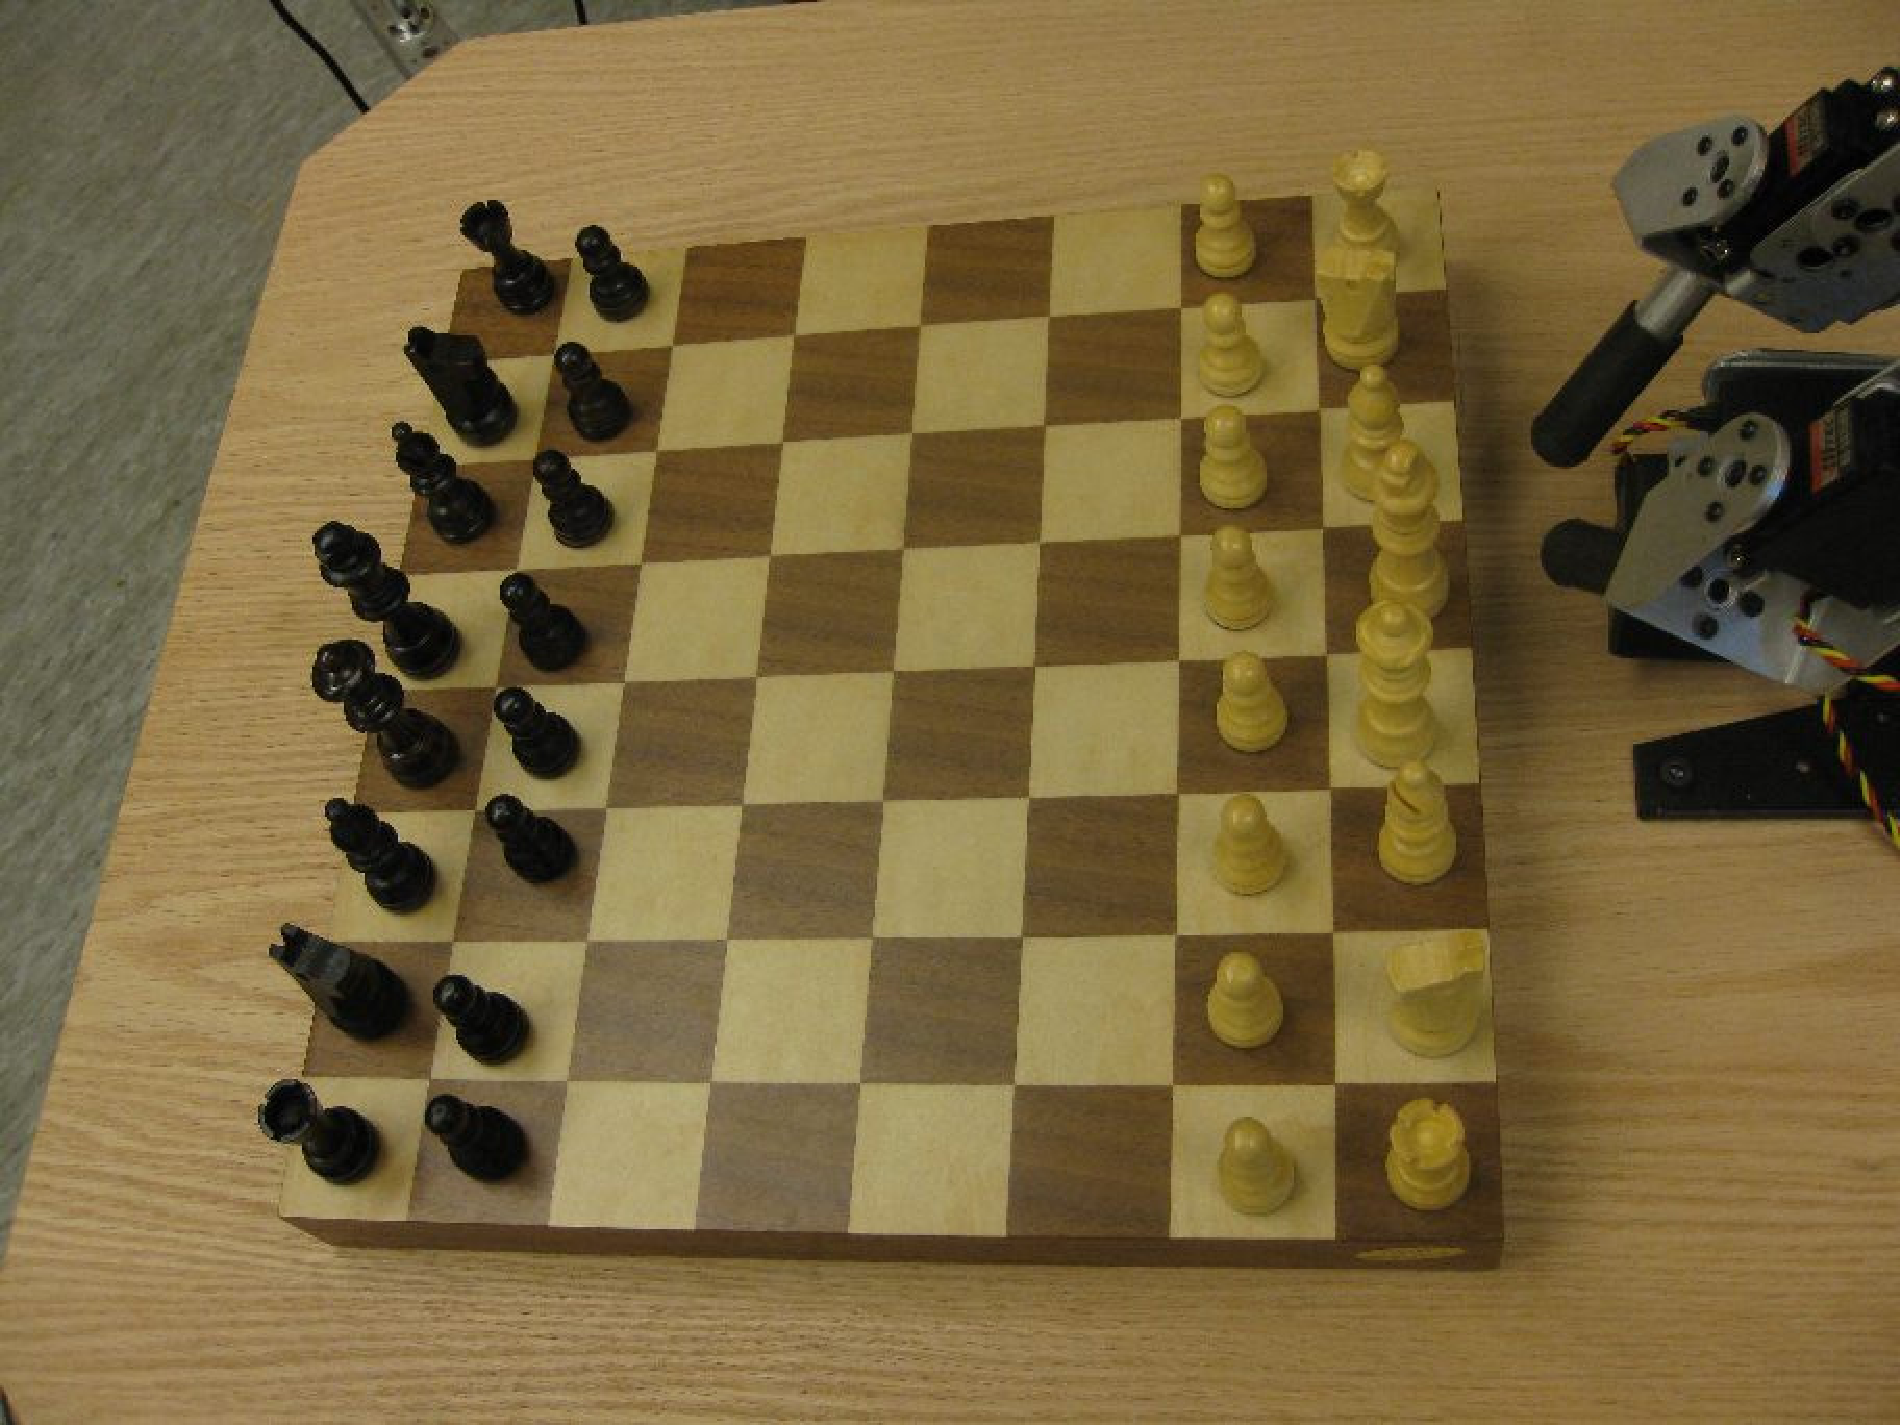
\includegraphics{chess}}\\
    	   	      \textsc{Game}
    	   	    \end{tabular}&
    	   	    \raisebox{5ex}[0pt][0pt]{\begin{tabular}{@{}c@{}}
    	   		plays\\
    	   		\scalebox{2}{$\longleftarrow$}\\
    	   	    \end{tabular}}&
    	   	    \begin{tabular}[t]{c}
    	   	      \resizebox{0.1\linewidth}{!}{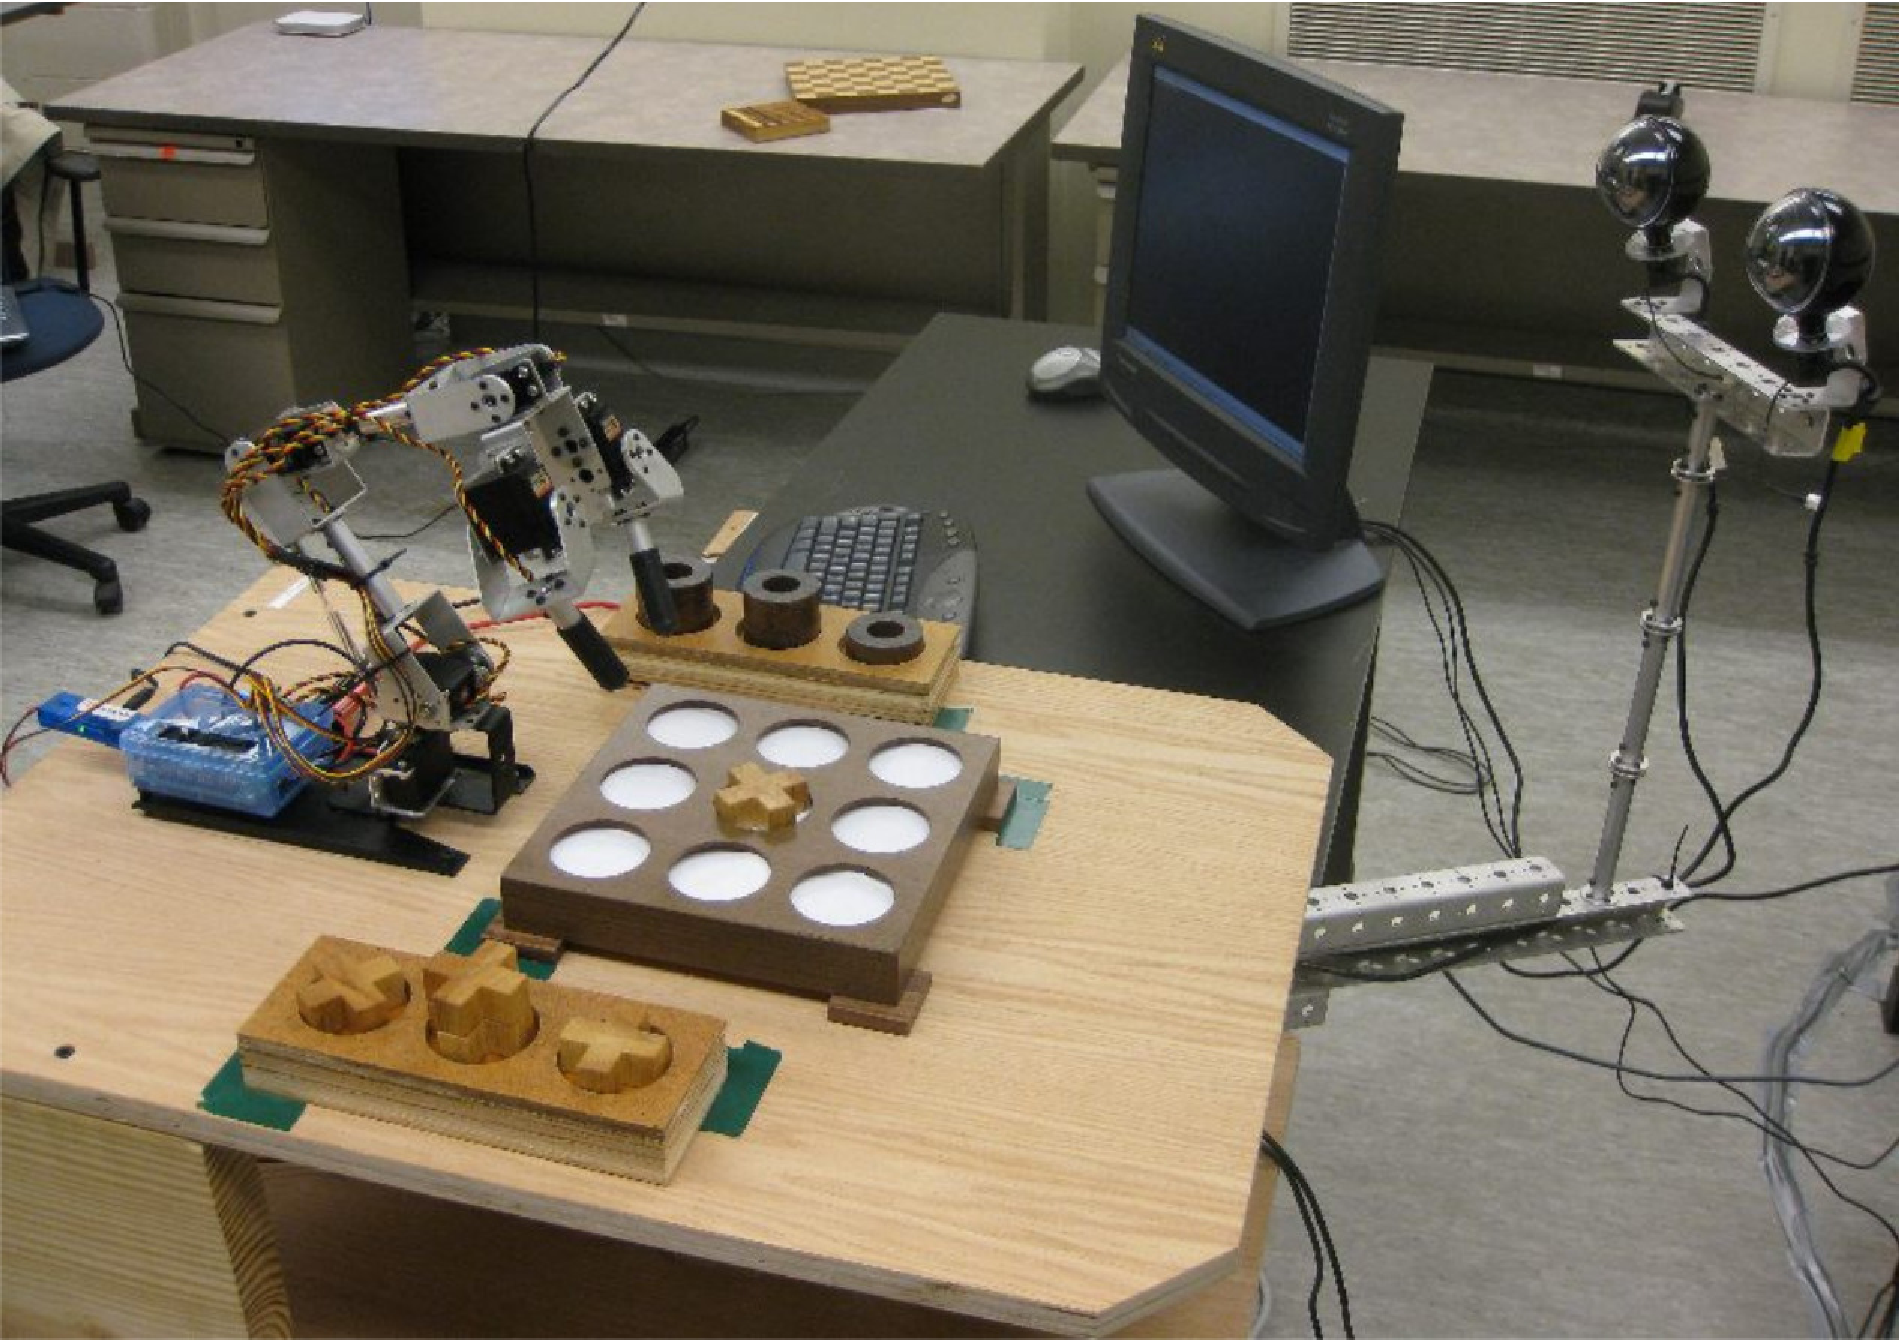
\includegraphics{orrorin}}\\
    	   	      \textbf{antagonist}
    	   	    \end{tabular}\\
    	   	    &&
    	   	    \scalebox{2}{$\uparrow$}\raisebox{1ex}[0pt][0pt]
		    {\makebox[0pt][l]{watches}}
    	   	    &&\\[1ex]
    	   	    &&\begin{tabular}[t]{c}
    	   		\resizebox{0.1\linewidth}{!}
			{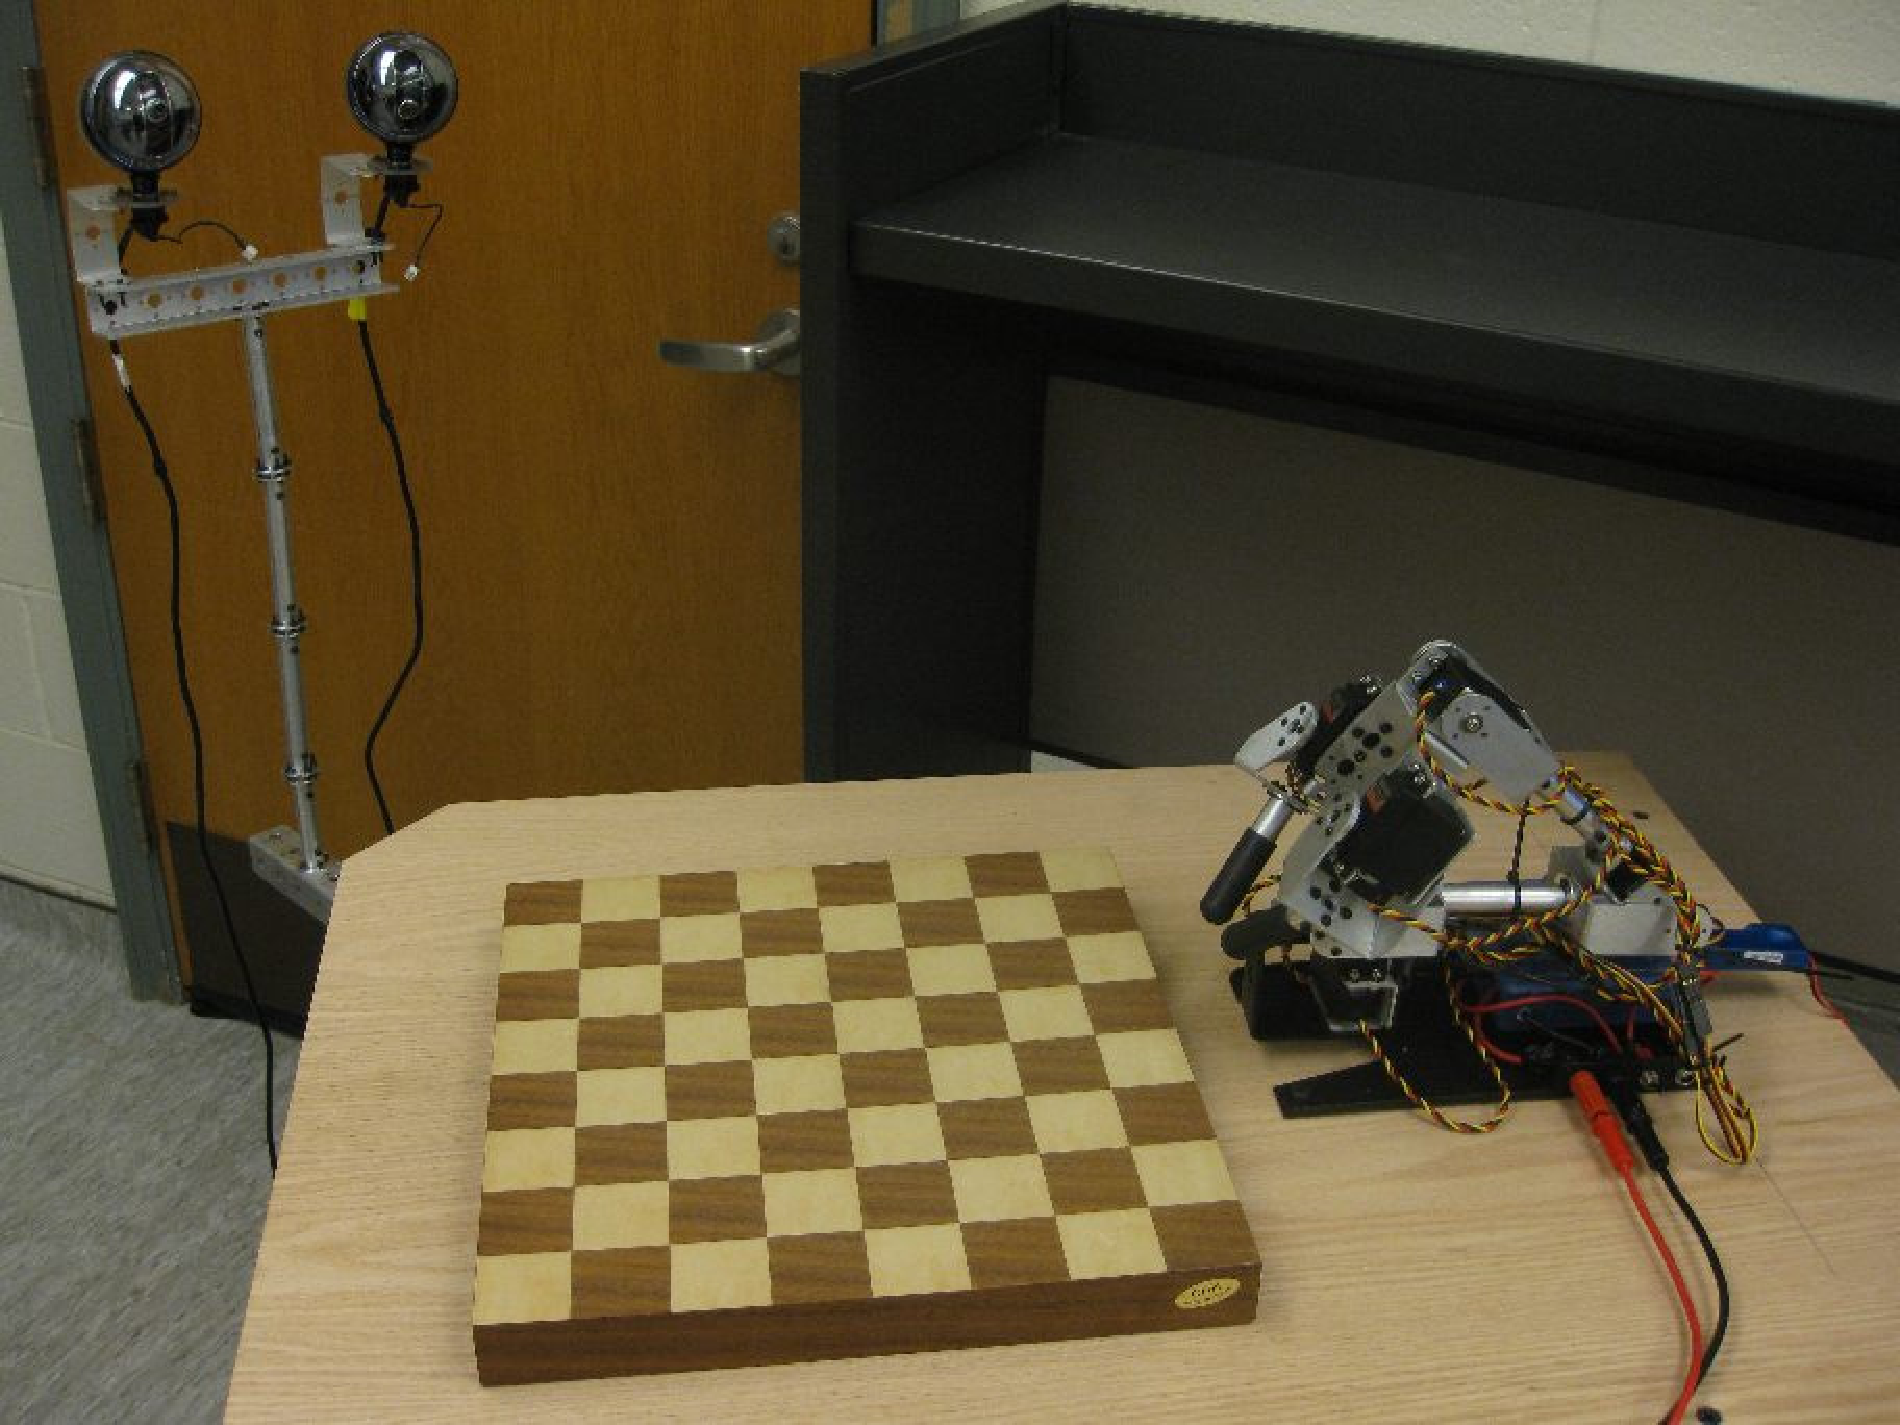
\includegraphics{tchadensis}}\\
    	   		\textbf{wannabe}
    	   	      \end{tabular}&&\\
    	   	  \end{tabular}\right\}&\Longrightarrow&
    	   	  \left\{\begin{tabular}{@{}c@{}c@{}c@{}c@{}c@{}}
    	   	  \begin{tabular}[t]{c}
    	   	    \resizebox{0.1\linewidth}{!}
		    {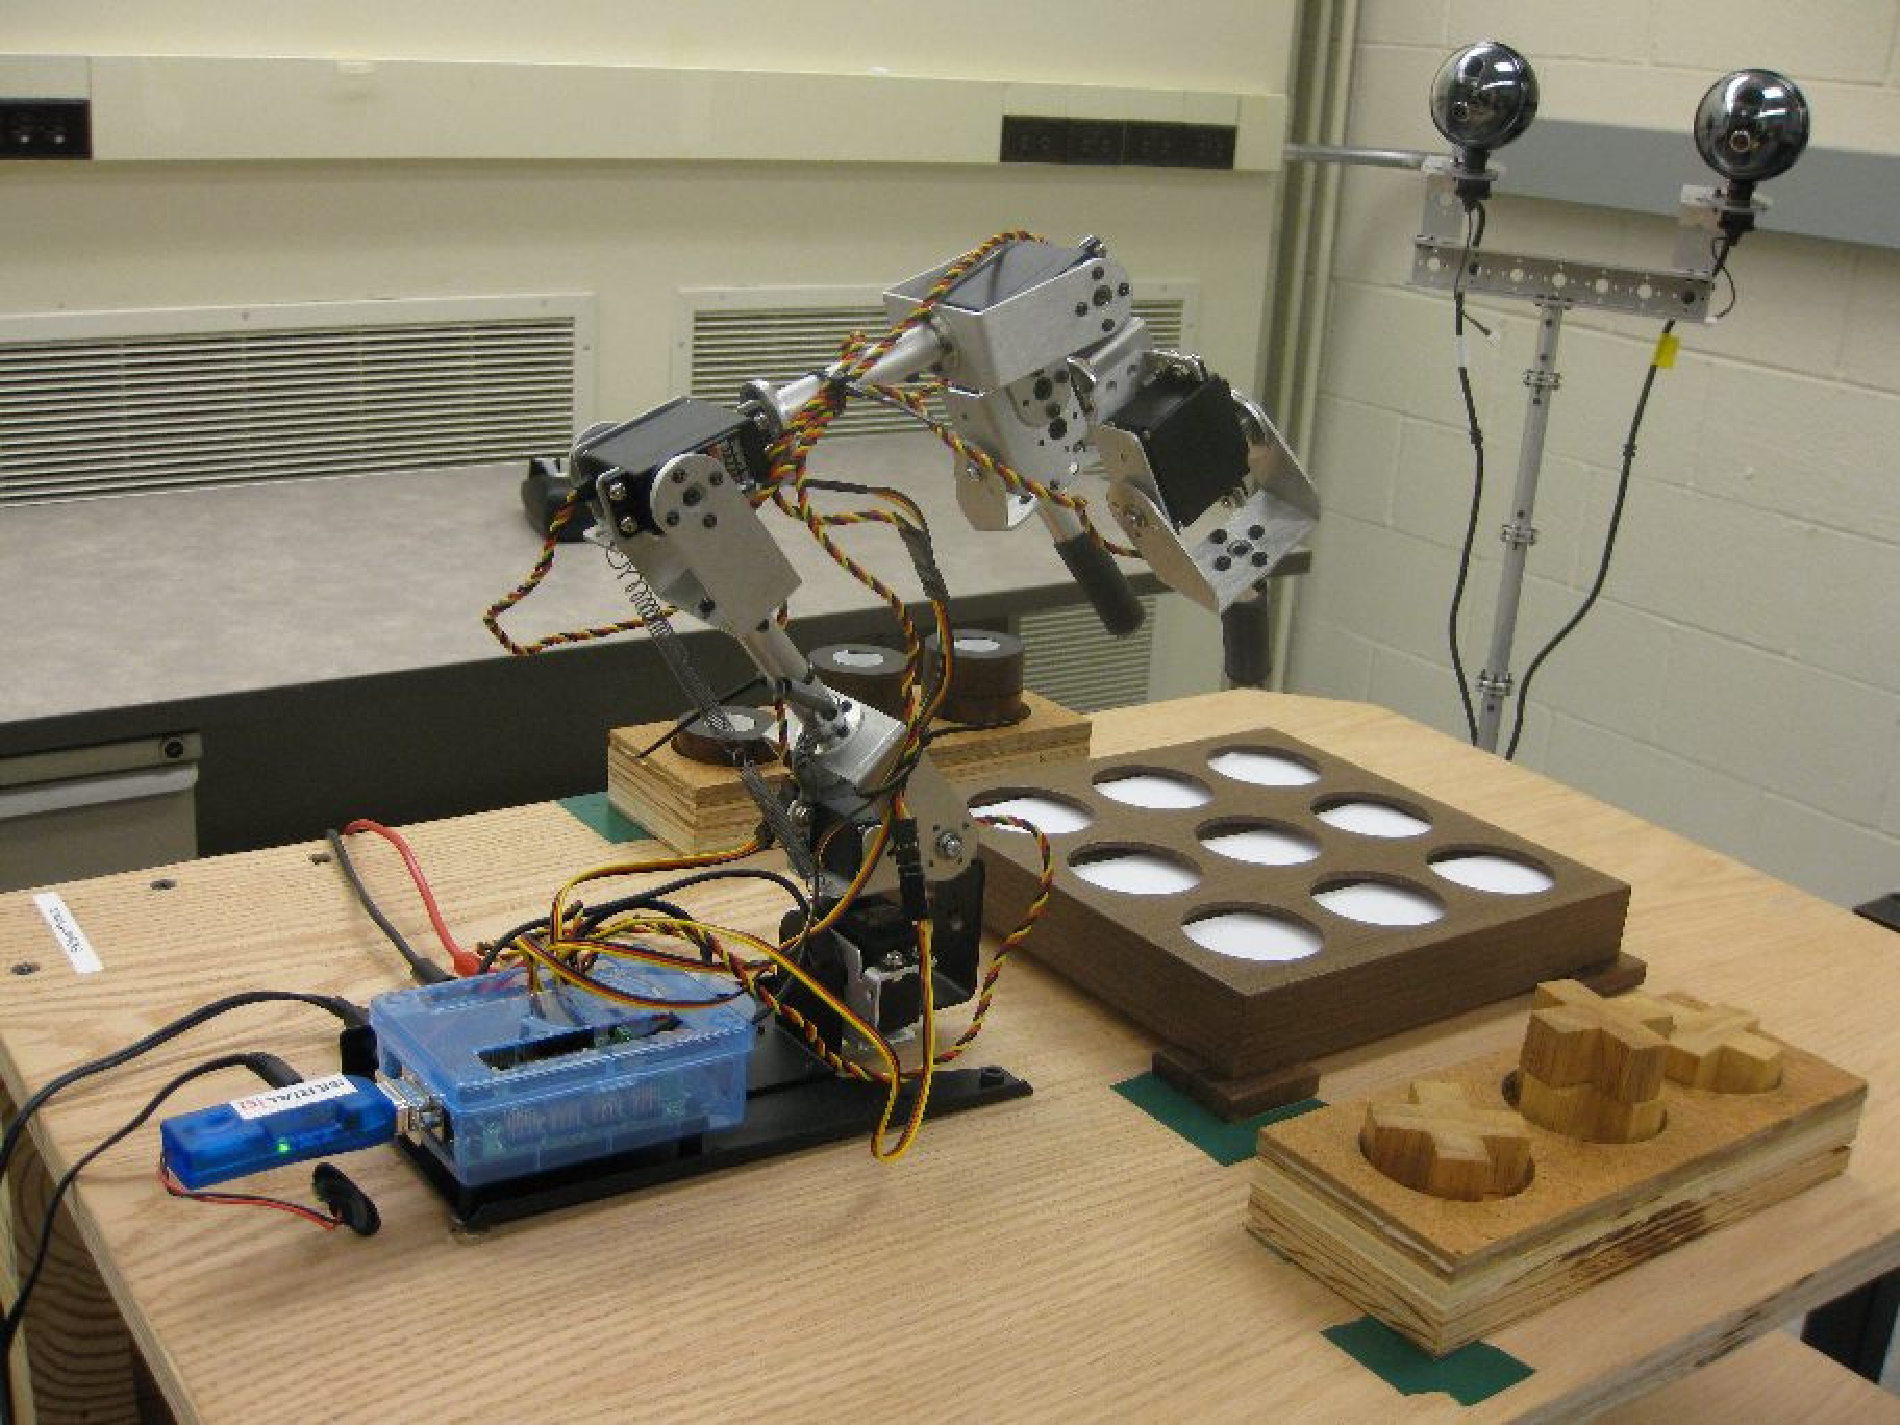
\includegraphics{sahelanthropus}}\\
    	   	    \textbf{protagonist}
    	   	  \end{tabular}&
    	   	  \raisebox{5ex}[0pt][0pt]{\begin{tabular}{@{}c@{}}
    	   	      plays\\
    	   	      \scalebox{2}{$\longrightarrow$}\\
    	   	  \end{tabular}}&
    	   	  \begin{tabular}[t]{c}
    	   	    \resizebox{0.1\linewidth}{!}{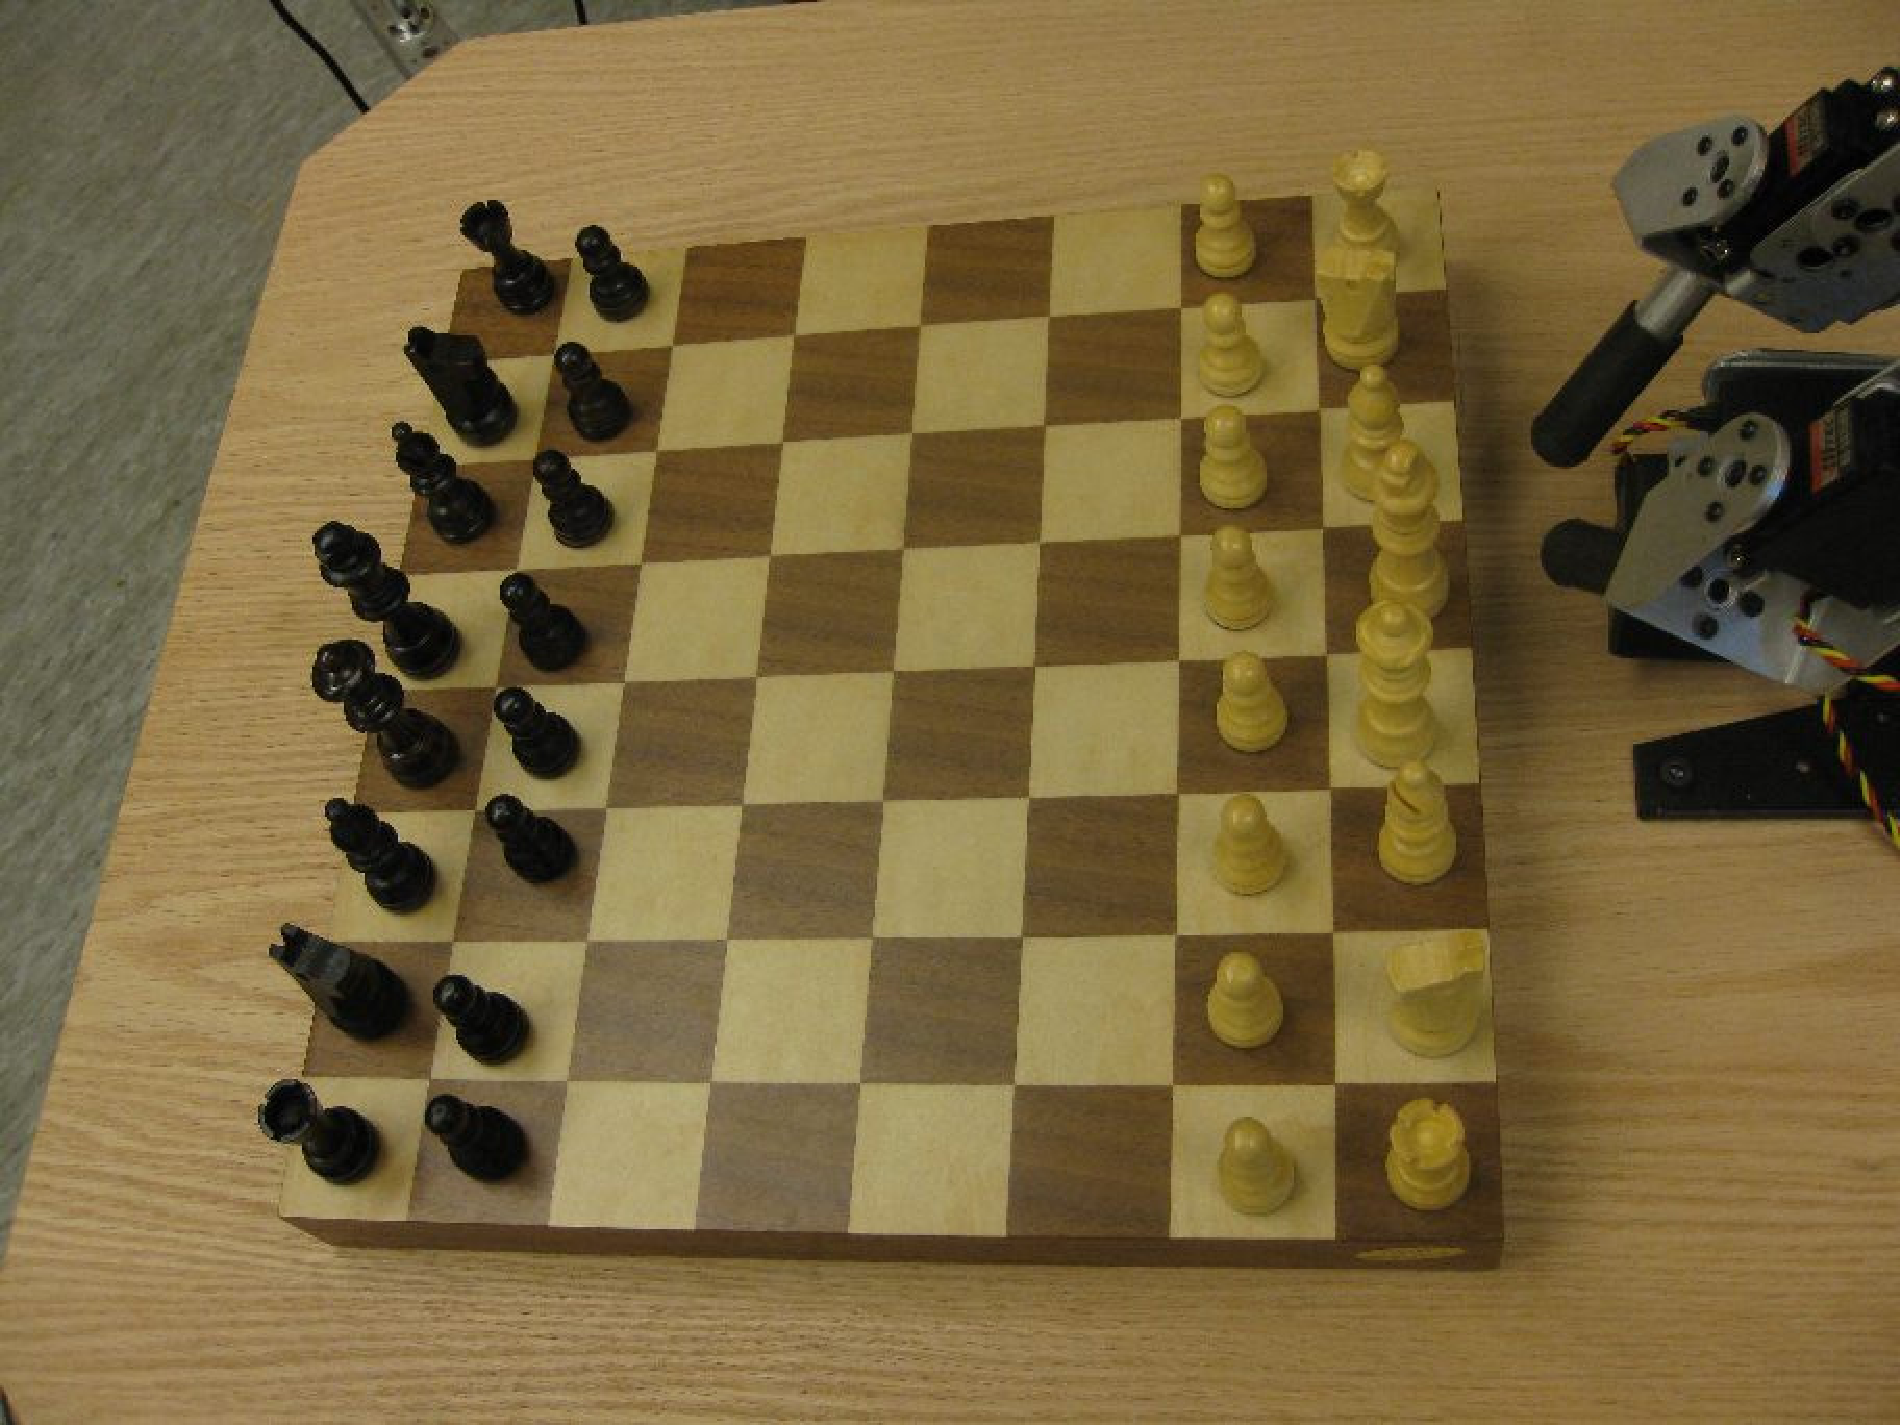
\includegraphics{chess}}\\
    	   	    \textsc{Game}
    	   	  \end{tabular}&
    	   	  \raisebox{5ex}[0pt][0pt]{\begin{tabular}{@{}c@{}}
    	   	      plays\\
    	   	      \scalebox{2}{$\longleftarrow$}\\
    	   	  \end{tabular}}&
    	   	  \begin{tabular}[t]{c}
    	   	    \resizebox{0.1\linewidth}{!}
		    {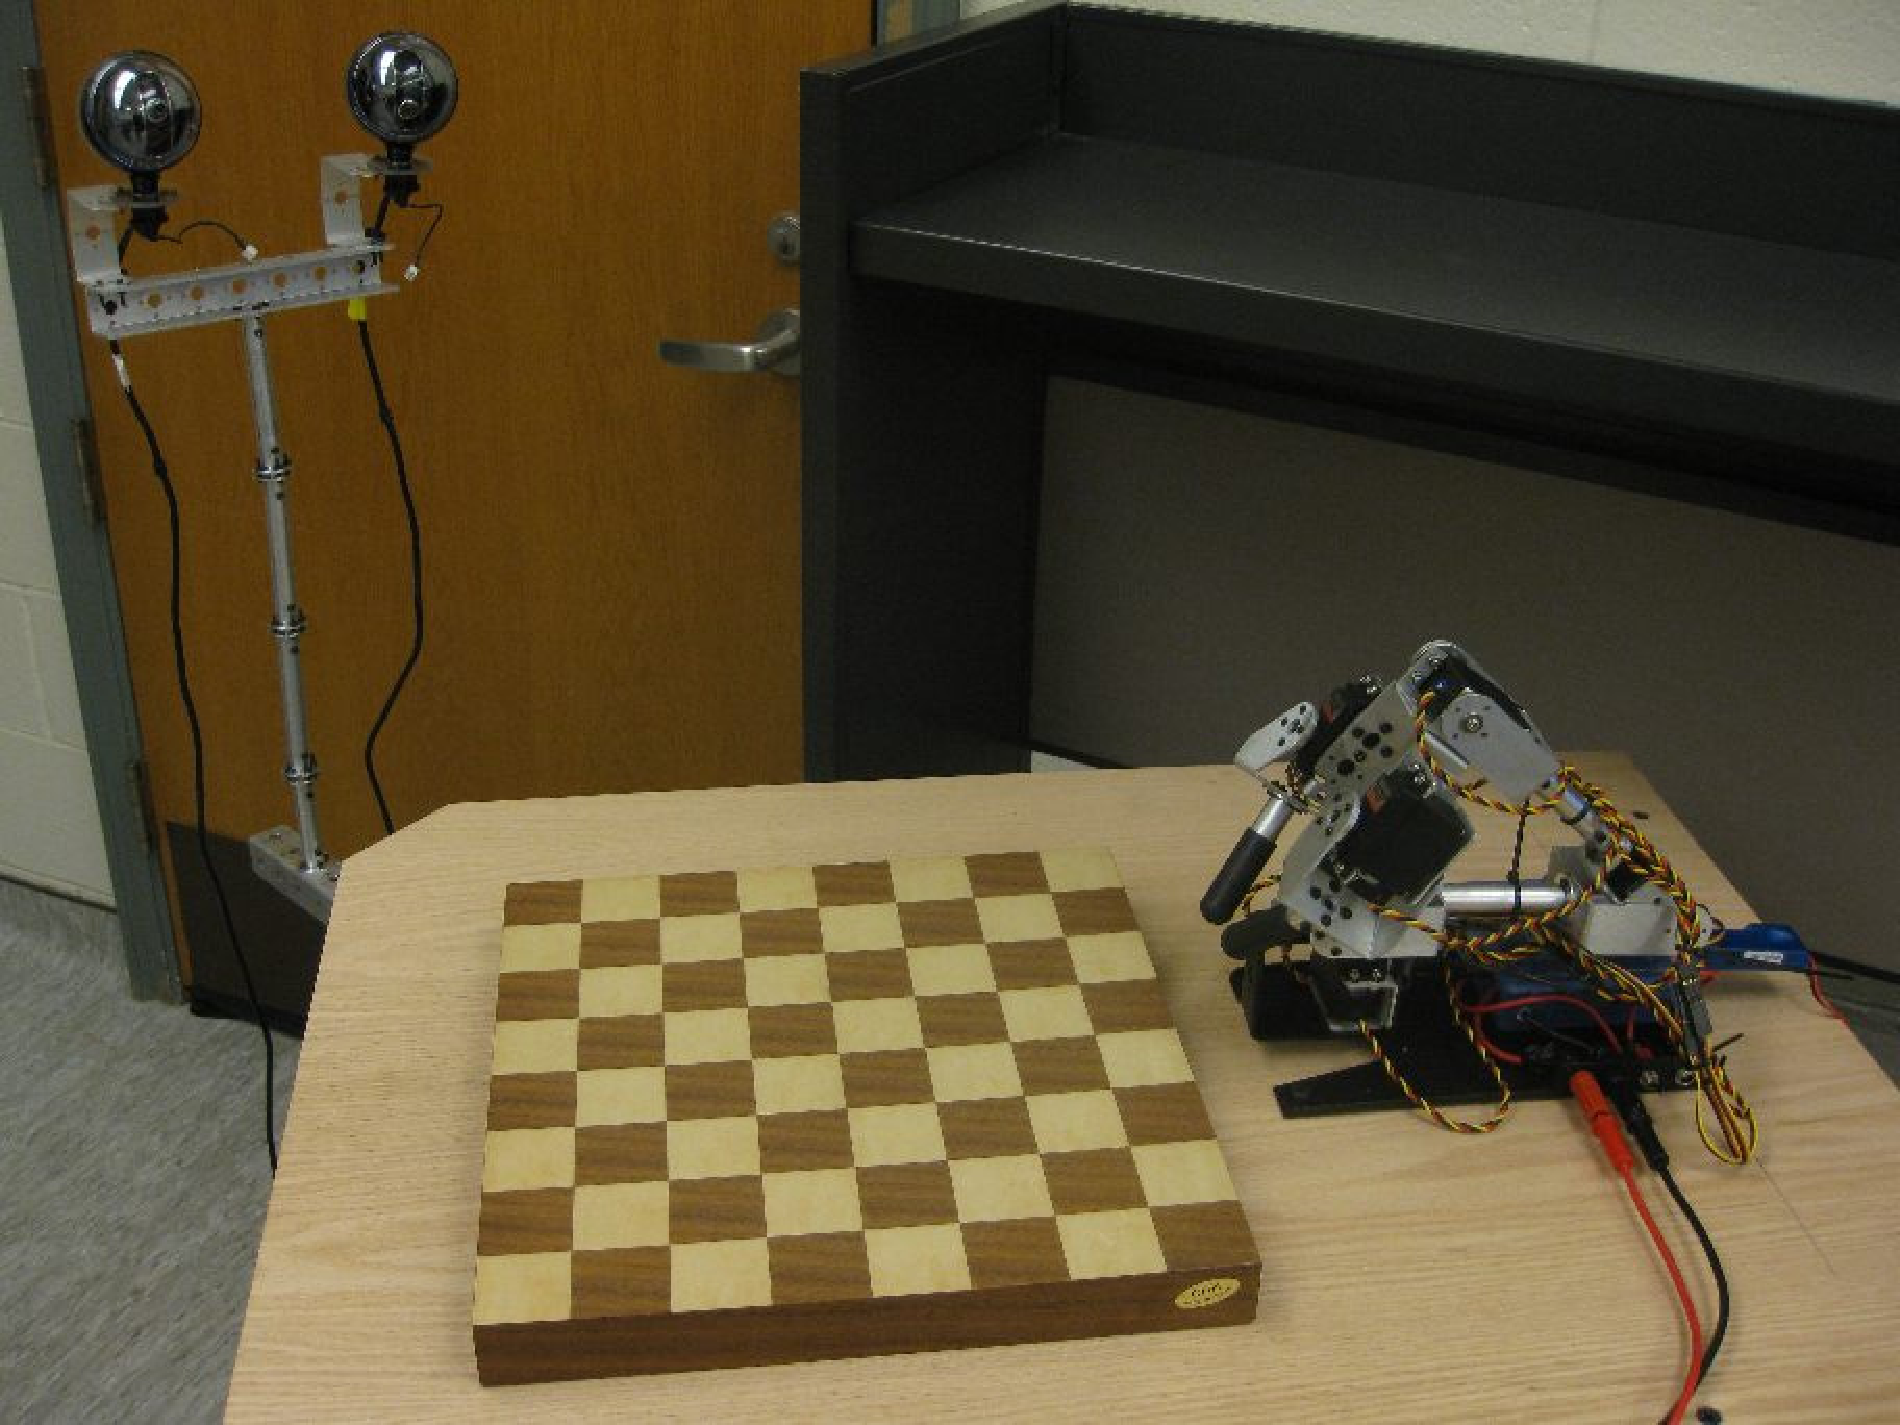
\includegraphics{tchadensis}}\\
    	   	    \textbf{wannabe}
    	   	  \end{tabular}\\
    	   	  &&&&\\[1ex]
    	   	  &&&&
    	   	  \begin{tabular}[t]{c}
    	   	    \resizebox{0.1\linewidth}{!}{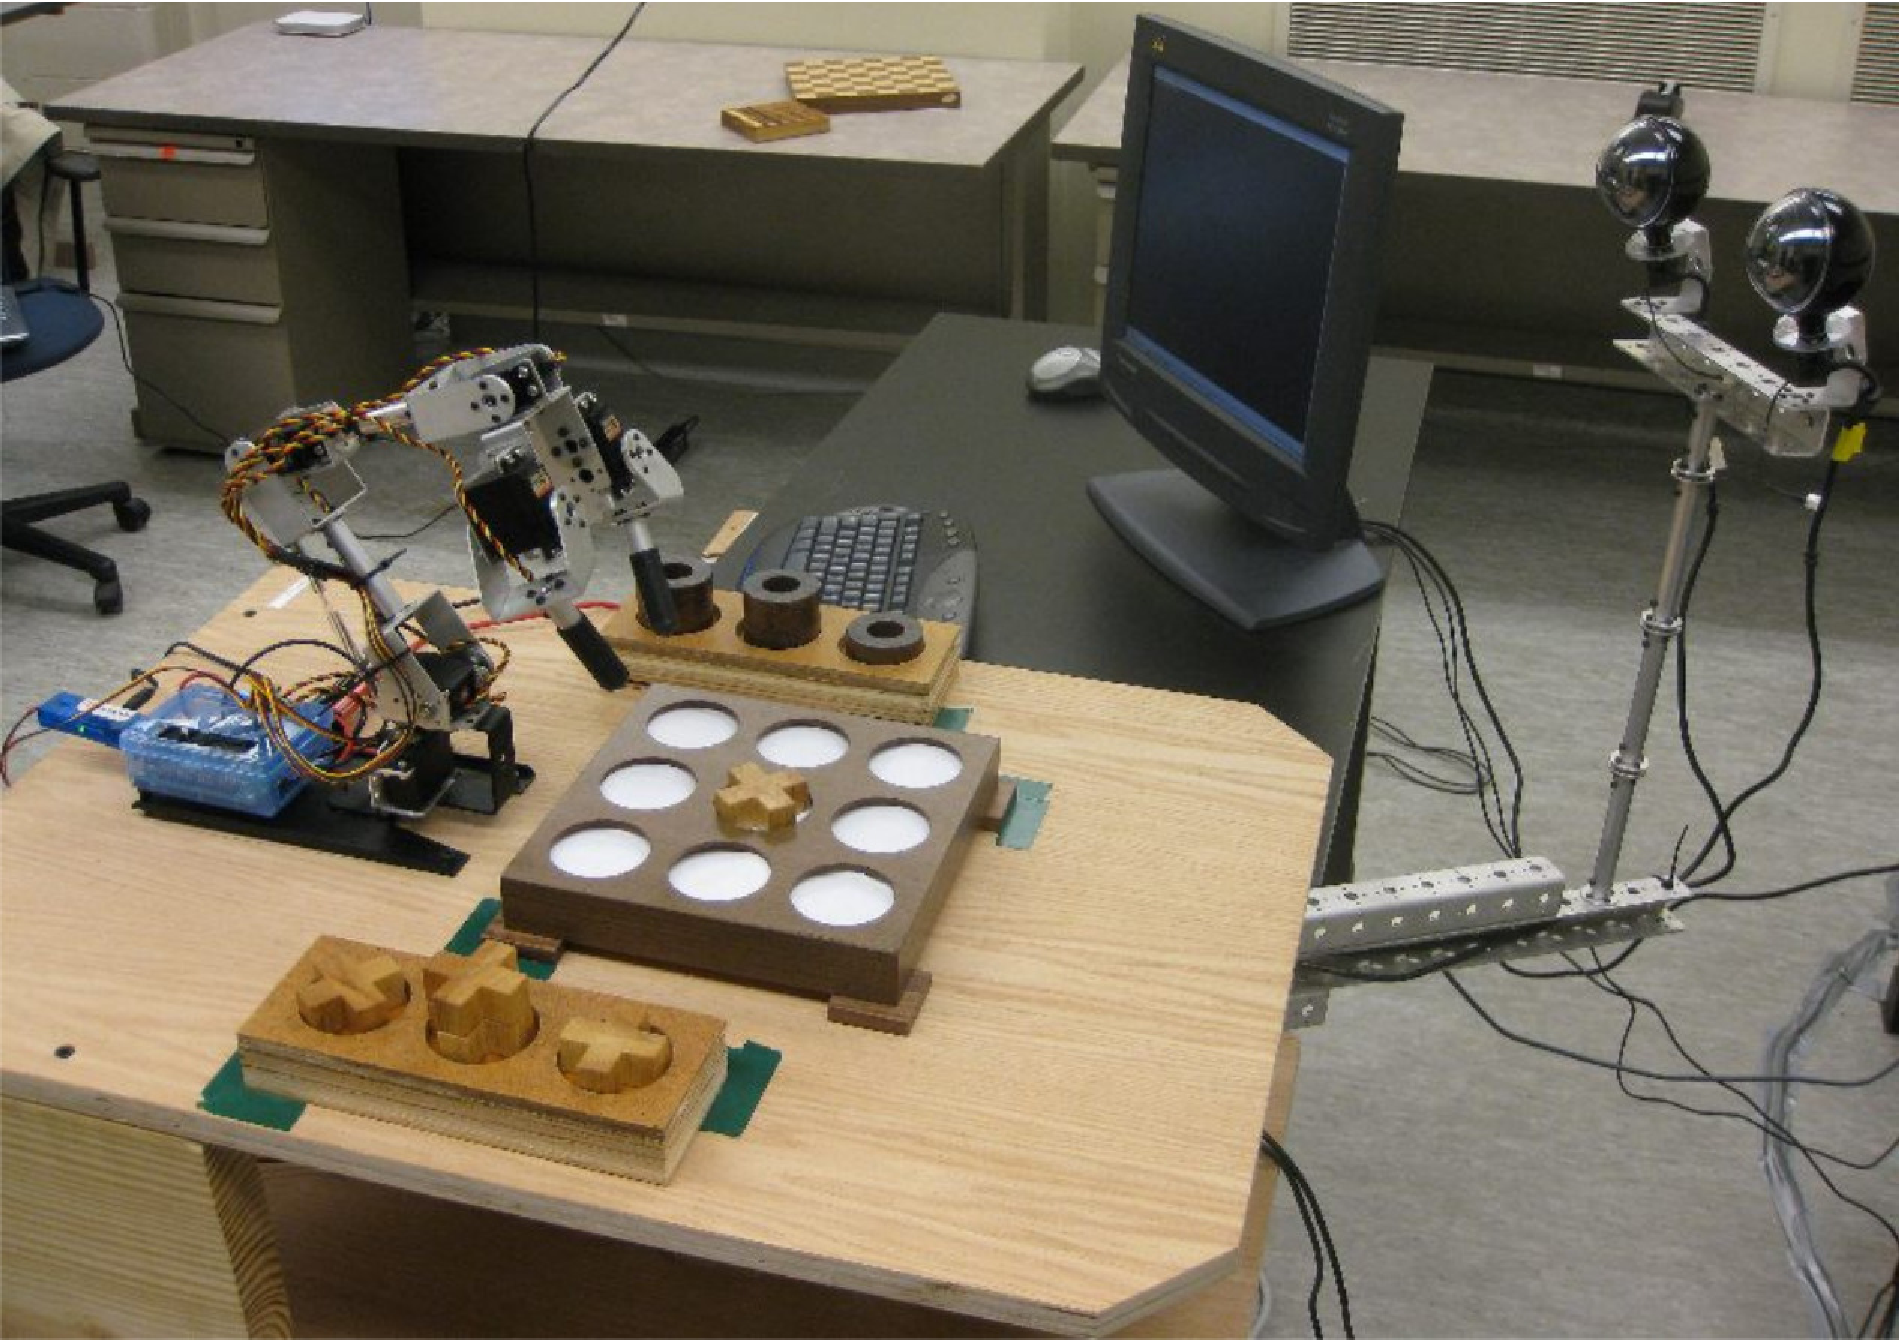
\includegraphics{orrorin}}\\
    	   	    \textbf{antagonist}
    	   	  \end{tabular}\\
    	   	  \end{tabular}\right.
    	   	\end{array}
	      \end{displaymath}
	    \end{center}
	  \end{scriptsize}
	\end{figure}
      \end{block}

      \begin{block}{Rules}
	\begin{itemize}
	\item \Progol, an inductive-logic-programming (ILP) system, is used
	  to learn the initial board, legal-move generator, and outcome
	  predicate
	\item rules represented as logical formulae, \ie\ Horn clauses
	\item learned rules are then directly executed with \Prolog
	\item system is given background knowledge about the world,
	  such as: a board exists, pieces can be on the board, players
	  own pieces, the concepts of linearity, forwards, sideways,
	  and the frame axiom
	\item background knowledge is of the type any child would have
	\item search the space of possible initial board, legal-move
	  generators, and outcome predicates for $3\times3$ games, given
	  the evidence of $n$ games, and find the most compressed rule
	  set which best explains the observed games
	\item learn the initial board first, then the legal-move
	  generator, and finally the outcome predicate
	\item use the previously acquired knowledge to learn the next
	  item
	\item can learn a full game description in a modest number of
	  games, typically 3--6
	\end{itemize}
      \end{block}
    \end{column}

    \begin{column}{.3\linewidth}
      \begin{block}{Results}
	\begin{itemize}
	\item reliable robust operation was achieved for 62 games,
	  approximately 2000 pick-up and put-down operations with
	  fewer than 20 interventions
	\item robotic manipulation based on dead-reckoning due to
	  non-linear relationship between servo control and angular position
	\item error detection by interleaving manipulation and visual
	  reconstruction of board states
	\item learned Hexapawn rule set:\\
	\scalebox{0.83}{\begin{lisp}
	    initial\symbol{95}board([[x,x,x],[none,none,none],[o,o,o]],player\symbol{95}x).\\
	    legal\symbol{95}move(A,B,C) :- row(D), col(E), owns(A,F), empty(G),\\
	    \ \ \ \ \ forward(A,H,D), at(H,E,B,F,I), at(H,E,C,G,J),\\
	    \ \ \ \ \ at(D,E,B,G,K), at(D,E,C,F,L), frame\symbol{95}obj(I,K,J,L,B,C).\\
	    legal\symbol{95}move(A,B,C) :- row(D), col(E), opponent(A,F),\\
	    \ \ \ \ \ owns(A,G), empty(H), forward(A,I,D), owns(F,J),\\
	    \ \ \ \ \ sideways(E,K), at(D,K,C,G,L), at(I,E,B,G,M),\\
	    \ \ \ \ \ at(I,E,C,H,N), at(D,K,B,J,O), frame\symbol{95}obj(L,N,O,M,C,B).\\
	    outcome(A,B,C) :- row(D), opponent(A,E), forward(E,D,F),\\
	    \ \ \ \ \ forward(E,F,G), owns\symbol{95}outcome(E,C), owns\symbol{95}piece(C,H),\\
	    \ \ \ \ \ at(G,I,B,H,J).\\
	    outcome(A,B,C) :- opponent(A,D), has\symbol{95}no\symbol{95}move(A,B), \\
	    \ \ \ \ \ owns\symbol{95}outcome(D,C).\\
	  \end{lisp}}
	\item learned similar rule sets for all 6 games
	\end{itemize}
      \end{block}

      \begin{block}{Lincoln Logs \& language}
	\begin{itemize}
	\item assembly task using assembly toys, \eg\ Lincoln Logs
	\item novel computer-vision system to recognize block
	  assemblies from grammars by extracting features, fitting
	  them to known grammars, and searching for implied necessary
	  or possible blocks
	\item novel language component to describe assemblies in terms
	  of walls and windows, and reconstruct the same structure out
	  of different assembly toys
	\item more advanced robotic system, with custom grippers,
	  farther reach, tactile sensors, and a palm-mounted camera
	\item more robust robotic manipulation using visual servoing
	\end{itemize}
      \end{block}

      \begin{block}{Future work}
	\begin{itemize}
	\item complete the Lincoln Log task and move on to other
	  assembly toys
	\item expand upon the current game learning and scale
	  up to games of higher complexity, \eg\ checkers
	\item learn the mapping from world state to game state
	\item learn Lincoln Log and other assembly-toy grammars
	\item integrate more sensors, \eg\ a laser pointer and
	  ultrasonic range finder
	\item stochastic ILP for fault tolerance
	\item a custom ILP system with better heuristics for learning
	  games
	\end{itemize}
      \end{block}

    \end{column}
  \end{columns}
\end{frame}

\end{document}

%%% Local Variables:
%%% fill-column: 79
%%% End:

% LocalWords: tex bibtex env BIBINPUTS BSTINPUTS TEXINPUTS american Stratego
% LocalWords: testbed tac sr ie UTF qid orrorin eps Hexapawn en passant pre
% LocalWords: dodgeball ilp Lynxmotion Logitech repurposed DOF USB QuickCam
% LocalWords: webcams pivotable conflate Xs ccc col obj OpenCV Progol inc dec
% LocalWords: int RI RROW CCOLUMN cvFitEllipse ab initio kinematically endgames
% LocalWords: Bradski Muggleton
